\begin{figure}[t]
    \centering
    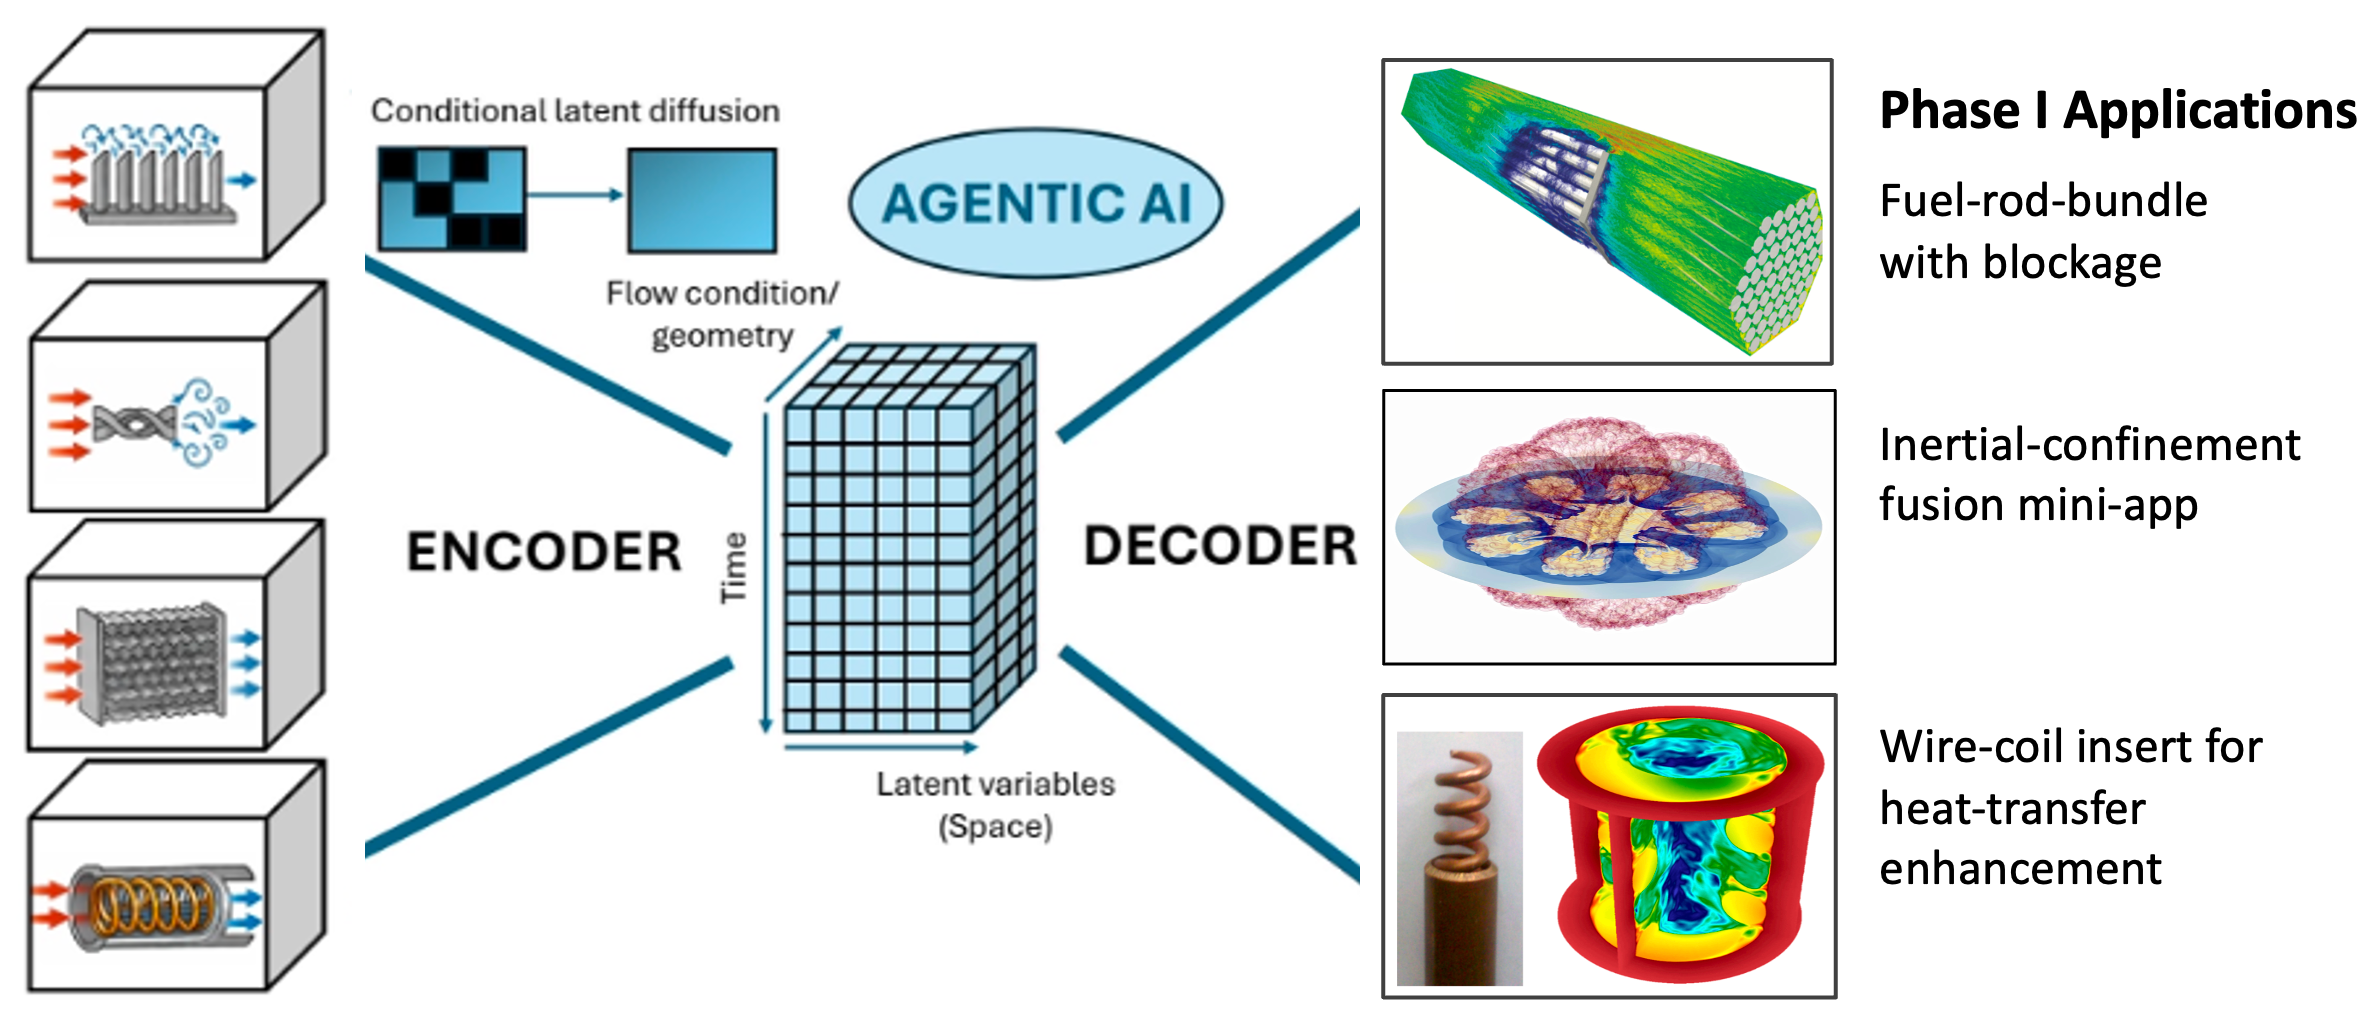
\includegraphics[width=0.48\linewidth]{../figs/method_w_labels.png}
\caption{
\small
Schematic of proposed method combining a foundation model with agentic AI.
Data-flow is left-to-right.  High-quality fluid-flow datasets
(e.g., mesh, solutions, QOIs) are used to train a foundation model, which
encodes all cases into a common latent space.  Conditional latent diffusion
is used to learn the distribution across cases in the latent space.
Spatio-temporal solution data for a new geometry can be quickly produced in the latent
space and decoded back to physical space.  The agentic AI framework has
access to this foundation model and the various optimizers, orchestrating a
significantly accelerated optimization/design process.
}
\label{fig:fm1}
\end{figure}
